

The goal of this introduction will be to give the reader a general initiation as to how economics treats property rights and how this relates to intellectual property. Most of the discussion is aimed at summarizing the relevant literature but some commentary is original. Section \ref{origins} delves into the roots of the debate and the modern legal language way of discussing such rights. Section \ref{static} aims to give some brief definitions of the kind of efficiencies economists concern themselves with, and to discuss how these notions apply to the Coase theorem and property rights. Dynamic aspects of property rights and incomplete contracts are elaborated in section \ref{dynamic}. Finally some comments on economic arguments of intellectual property are reviewed in section \ref{intellectual}.

\section{The origins on the debate about private property} \label{origins}

The roots of the debate about property rights originate from Ancient Greece through its two most revered philosophers, Plato and Aristotle. 
Plato's most famous work, the Republic, is a treatise on an idealized society, one that has managed to halt to a minimum its own deterioration from the perfect form. Plato's view of property rights is purely instrumental in that it is something that will help maintain the ideal society from deteriorating. His conception of ownership is as an important source of corruption that creates clannish self-interest and considers the panacea of this influence to be the abolition of private property. Aristotle takes a stand against Plato, his former teacher, in being one of the first defenders of private property. In "Politics",  Aristotle reasons that without private property people would interfere in each other’s affairs without being motivated by love. He views the act of waiving your rights to property against an individual as a way to be virtuous. Consequently, a limitation of this right would limit the ability to be virtuous. The debate between Aristotle and Plato has echoed for millennia, with various philosophers taking different sides of this debate. For instance, Hegel defended property rights based on his theory of person-hood, stating that people are defined by their will and the only way to manifest their will is through physical objects. Philosophers even had views on intellectual property. Hume for instance, claimed that property should be placed on only goods which are scarce\footnote{see \cite{plant1934economic} for views of various philosophers}.

Perhaps the most influential modern non-economic normative view of property is John Locke's theory of 'homesteading' \footnote{\cite{locke2014second}}. Locke's view of property rights is as a method of linking a person who is creating value to that value. This is done by mixing one's labor with the object or land which makes the physical object inseparable from its founder. The view is often rather vague as it does not distinguish between the different amounts of value added and the scope of homesteading. 

Economics has always focused not on the origins of property, but on its effects. Using this lens, perhaps the most famous critic of the Lockean theory of property was Karl Marx who claimed the opposite, that private property is the means by which workers become alienated from their labor. The logic behind this is rather simple: if an employee adds a number of hours’ worth of labor, he will necessarily be compensated less than that number of hours’ worth by the property owner otherwise there would be no way of making profit, hence exploitation. This is one of the first views of property which focused on its dynamics. Specifically here, the dynamics on wealth inequality. However these kinds of interpretations have been superseded as value has been associated not with only inputs but by the tastes of agents and the relative scarcity of resources. Similarly, profit could be entirely explained by other factors such as the relative advantage firms have in information, whether it be an edge in production, taste, impulses of consumers etc. This does not entail that property is disconnected from value, merely that value is not caused by labor, though it is correlated.

Perhaps the first fully prescriptive system of property was articulated by Henry George \footnote{\cite{progress}}. His system aims to reduce some of the dynamics described by Marx. George devised a system where property is temporarily allocated to the highest bidder. What is ingenious about the modern version of the Georgist scheme is that it aims to eliminate land rents by making tenants bid for their own rents. This creates a system where people will only earn their labor rent and not the land rent of value. The most known response to this is the view of Hayek\footnote{\cite{Fatal}}. In this view the function of property is not homogeneous across individuals and making ownership temporary is prescriptive in not only the system of property but also in what agents should pursue. For instance, if an agent uses land to pursue non-monetary goals, the tendency will be for that agent to be replaced by an agent who pursues monetary goals since those goals will be aligned much closer with the ability to bid. In other words, the effect of the property system is not simply to allocate goods efficiently but to allow agents to discover their own goals. 

%Structure of production not clear,

\subsection{What is a property right?}

A tentative answer to this question is\footnote{The presentation borrows from \cite{Munzer1990}}: property is simply the default contract. That is, if people do not agree on a contract, property is what is taken as the baseline. 'Property as the default' view is simple enough: Person A can contract with person B that person B will not touch or use item z without A's permission. This in fact, requires no property right at all. What does require a property right is that all other people will also not be able to do with z as they please. If agents could all simultaneously consent or if there were solely two agents who could contract, there would be no need for property rights. Indeed, property rights rely on the inability to contract or simply the costliness to contracting with all agents simultaneously. This basic reasoning is the motivation behind incomplete contracting (which is discussed in section \ref{incomplete} ).


\subsection{The language of property rights}

\begin{figure}
\begin{center}
%\begin{tikzpicture}[every text node part/.style={align=center}] used for multiple parts,
%along with shapes.multipart tikz library.
\begin{tikzpicture}[sharp corners=2pt,inner sep=7pt,node distance=.8cm,every text node part/.style={align=center}]

\node[draw, minimum height = 3cm, minimum width = 3cm](Privilege){\textbf{Privilege:} A can use \\ \textcolor{blue}{ \textbf{Power:} A can change B's  rights}};
\node[draw,below=2cm of Privilege, minimum height = 3cm, minimum width = 3cm](Duty){\textbf{Duty:} A has no right to use \\ \textcolor{blue}{\textbf{Disability:} A can't change B's rights}};
\node[draw,right=2cm of Privilege, minimum height = 3cm, minimum width = 3cm](No-claim){\textbf{No-claim:} B cannot exclude A\\ \textcolor{blue}{\textbf{Liability:} B's rights can be changed by A}};
\node[draw,below=2cm of No-claim, minimum height = 3cm, minimum width = 3cm](Claim){\textbf{Claim:} B can exclude A \\ \textcolor{blue}{\textbf{Immunity:} B's rights can't be changed by A}};

%Draw arrows
\draw[-triangle 90, ultra thick,<->] (Privilege) -- (Duty) node [midway, above, left = 0.1cm]{opposite:};
\draw[-triangle 90, ultra thick,<->] (Privilege) -- (No-claim) node [midway, above]{correlative:};
\draw[-triangle 90, ultra thick,<->] (No-claim) -- (Claim) node [midway, above, right = 0.1cm]{opposite: };
\draw[-triangle 90, ultra thick,<->] (Duty) -- (Claim) node [midway, above]{correlative:};
%\draw[-triangle 90, ultra thick,<->] (Privilege) -- (Claim) node [midway, above, rotate = -45]{$\mu^{03}_{x+t:y+t}$};
\end{tikzpicture}
\caption{First order rights, \textcolor{blue}{Second order rights}}
\end{center}
\end{figure}

The most basic method of discussing property rights is by using jurist language\footnote{See \cite{Hohfeld}}. Discussions of rights are separated into different hierarchies but in most applications only two levels are needed. 

First order rights, which describe the direct rights an agent possesses, are usually the positive rights to act on an asset or to exclude another agent. The right to use is called a "privilege" and the right to exclude is called a "claim". These rights are zero sum in the sense that if all agents have a "privilege" then no agent has a claim. On the other hand if at least one agent, agent B, does not have a "privilege", then  agent B has a "duty" and there is some set of agents, A, who either individually or collectively (perhaps democratically) have a claim against B.

Second order rights dictate the use of first order rights. For instance, when one talks of "power" this is in reference to the right to transfer, waive or annul "claim" and "privilege" rights. For instance, the right to change who can use the property is a second order right. One can also speak of "immunity", which means that one has the right for his "claim" or "privilege" to not be affected by others. Second order rights are about how first order rights can be changed. The possibility space of first order rights is increasing in power and decreasing in immunity. Second order rights may also have the feature of circularity; Agent A may have power over B; B may have power over C; and C may have power over A.

Notice that if an agent has power over an object, this entails the ability to control someone's first order rights. Both first order and second order rights may be under negotiation in contracts. The arrangements that can legally emerge are much narrower without power. However, second order right do not entail the right to destroy or abandon an object. The right to destroy or abandon requires \textit{infinite order} rights. This is because the destruction and abandonment of an asset implies that all other agents use and power rights on the asset are violated. Even if all the power rights were centralized on a single agent, this still does not entail the right to destroy or abandon. This is due to the fact that we also have to consider who has the rights to change power (a third order right). And this reasoning can be applied recursively, hence the right to destroy and abandon entails infinite order rights\footnote{For an interesting analysis of the right to destroy/abandon see, \cite{Strahilevitz2005}, \cite{Strahilevitz2009}}. 
%think about adding things here

%When does someone have the right to abandon or to destroy? 

The contractual possibility of first order rights depends on the distribution of claims or privileges. If all agents have privilege rights on an asset then this naturally entails that the only contracts agents can draw are either committing to using or not using the asset. If on the other hand an agent has claim rights on an asset, then that agent can also contract the exclusion of other agents from using that asset. If cost is independent of the number of agents one is contracting with, then there is no advantage to uniting claim rights upon a single individual. However, if approaching each agent is costly then it may be advantageous to allocate claims to a single agent. While the contractual possibility space is entirely available in all cases, the property right regime can achieve the same contractual space with fewer parties. Similarly, the types of arrangements possible (corporations, partnerships, non-profits, licenses, bailments, non-voting common stock, trusts, agencies, employee-employer relationships, marriages, etc) entirely depend on second order rights. With this in mind, we clarify how some property right paradigms fit into this conceptual framework.

To clarify ideas it is useful to know how this taxonomy matches with traditional economic ideas. For instance, clearly if there is a law that requires property owner A to allow access to B, this implies that agent B has a privilege of use, and implies that A has a no-claim. Similarly, this implies that B has immunity and A has a disability. A price control is a limitation on what price one can sell their good for. As such, it is a "power" limitation in the sense that without a price control A could transfer the asset on wider terms.

The above puts a heavy emphasis on 'use' and 'exclusion', however the notion of 'use' in the case of land is a broad term that encompasses numerous rights that are separable. The additional rights that can be constructed from 'use' are: access, the right to freely move within that territory; management, the right to control the internal organization of the land; withdrawal, the right to extract things from the land; alienation, the right to sell or lease\footnote{\cite{ostrom2010private}}.
Land ownership specifically has been summarized by the simple hierarchical relationship corresponding to the five rights, $\text{authorized entrant} \in \text{authorized user}  \in \text{claimant}  \in \text{proprietor} \in \text{owner}$ (each level of the hierarchy adds a right). \footnote{See \cite{schlager1992property}}


The two natural limits to the jural taxonomy are when only the state has second order rights and sovereignty. One possibility for the absence of a second order right is that all agents have privileges, this is termed \textit{Open access} (open sea and atmosphere or explicit prevention of exclusion zones). Alternatively, the absence of second order rights could be when the state allocates claim or privilege rights to a specific group. This could look like a king choosing vassals or democracy selecting managers. \textit{Sovereignty}, on the other, hand implies that someone has infinite order rights. If someone has the capacity to make someone else an owner, this can only be represented by an infinite recursion. However, the specific scope of ownership will depend on the regulations in place. The scope of ownership has often been articulated as "the right to do with your property as you wish as long as nobody else is harmed by it". However, such definitions are problematic as the notion of harm can be interpreted in a variety of ways. A simple solution to this looseness is to revise the definition to "the ability to use ones property in any way one wishes as long as the \textit{physical} characteristics of others property is not affected" \footnote{\cite{Alchian1965}}. Notice that this definition is not free from interpretation because the notion of 'physical' is not clear (for example: a change in air quality). However once the notion is adopted it creates an objective measurable standard that is open to external verification. We define the word \textit{intrusive} in this physical sense.
%improve, not clear what sovreignty


\newpage
\textit{Private property} is often a term used to describe some kind of constrained sovereignty. While both sovereignty and private property imply infinite order rights on the set of rights granted, the set of rights granted by private property is smaller. Private property does not entail that the owner has higher order rights on all possible uses. If we imagine the three sets below, private property implies simply that $B \cap C$. Private property is sovereignty in the special case where $B\cap C=C$. These relationships are summarized in figure 2.


\begin{align*}
A:=\{ \text{Possible uses of an asset} \} \\
B:=\{\text{Non-intrusive uses} \} \\
C:=\{\text{Uses on which privilege is granted}\}
\end{align*}




\begin{figure}[hb]
\begin{center}
%\begin{tikzpicture}[every text node part/.style={align=center}] used for multiple parts,
%along with shapes.multipart tikz library.
\begin{tikzpicture}[ spy using outlines={circle,
  magnification=1, size=1cm, connect spies}]
 % Let's draw the scene (to magnify):
  \begin{scope}[spy using outlines=
      {magnification=16, size=8cm, connect spies, rounded corners}]

    % the boarder:
    \draw[thick, rounded corners] (-7,-6) rectangle (7,6);
    %\draw (0,6) node[scale=2] {Asset Universe};

    % The transparency:
    \begin{scope}[fill opacity=0.5]
      \fill[yellow] \firstcircle;
      \fill[blue] \secondcircle;
      \fill[red] \thirdcircle;
    \end{scope}

    % letterings and missing pieces:
    %\draw (0,-2) node {Possible uses of an asset};
    \draw (-4,3) node { \textbf{B} };
    \node[text width=2.1cm] at (-4.25,1) {\textit{Non-intrusive privileges not granted}};
    \node[text width=2cm] at (4.2,1) {\textit{Intrusive privileges granted}};
    \node[text width=2cm] at (0,1) {\textit{Non-intrusive privileges granted}};
    \draw (3.5,3) node {\textbf{C}};
    \draw (0,-4) node {\textbf{A} };
    %\draw (-4,2) node \text{Boom \\ A };
    \draw[align=center] \firstcircle node {};
    \draw[align=left] \secondcircle node {};
    \draw[align=center] \thirdcircle node {};
    \fill (-4.5,-0.5) circle (0.000)
        node[scale=0.04, align=center] {Intellectual\\ Property\\is possible};
    \fill (-1.5,-4.5) circle (0.000)
        node[scale=0.04, align=center] {Intellectual\\ Property\\is possible};

    % now we can draw the magnifying glass:
    \spy [circle,cyan, size=1.9cm] on (-4.5,-0.5) in node [left] at (7,0);
    \spy [circle,cyan, size=1.9cm] on (-1.5,-4.5) in node [left] at (6,-3);
  \end{scope}
\end{tikzpicture}
\caption{ Intellectual property is only possible if a privilege is not granted }
\end{center}
\end{figure}

\textit{Communal/Public property} on the other hand gives a subset of agents in society the right to use but not the right to exclude. Power is also given to a subset of agents. For example, this may be some community that aims to allocate fishing or hunting rights.
However, since alienation or transfer is limited, this generally implies higher order rights are in the hands of the state. The distinction between communal and public ownership is how the government chooses to exercise its higher order rights. If they are exercised for the sake of public servants, such as military reservation, then it is called "public" and if not we call it "communal" \footnote{For a discussion of using common property as a policy tool see: \cite{ciriacy1975common}}. The word "communal" usually also implies that there is some kind of privilege that agents have over the land. In the limit, as the set of agents who can exclude is empty, communal property becomes \textit{open access property}. In general, any regime with weak claim rights is a first come first serve type of property and agents operating in such a regime ignore the cost of use \footnote{\cite{Alchian1973} mentions how the Canadian government in 1970 set an upper limit to the number of seals to be clubbed which caused speed of hunting to be the competitive trait leading to over-hunting}.

There are other types of regimes which are less commonly discussed such as the \textit{Georgian system of property}. The Georgian system of property temporarily grants first and second order rights to individuals for a given period of time conditional on the individuals having the highest bid. Since ownership is temporary, and no permanent right is possible, this implies no higher rights than third order rights. Additionally, agents no longer have the right to transfer ownership since the decision to keep ownership temporary and conditional on winning the auction is ultimately given to the state.

%new
One way of presenting economics is as being the analysis of exchange. Adam Smith's two books are said to be about two notions of such an exchange; personal exchange and commercial exchange. These two notions correspond closely to the hierarchy of rights. To give a gift or to share something is within the sphere of personal exchange, as such agents need only have first order rights. Commercial exchange on the other hand is about impersonal exchange. Such exchange is conditional, and subsequently depends on, the ability to contract. The ability to contract on assets requires higher order rights. Hence, the degree to which a society can become a commercial society depends on how higher order rights are distributed. 

The language presented is especially interesting for the analysis of intellectual property. Whilst each physical property can be seen as a list of rights and the matching of those rights to individuals or groups of individuals as described above, the concept of intellectual property is qualitatively different. The notion of intellectual property is a limitation of the first order rights of "privilege" on physical property. That is, if one has intellectual property on the concept of a wooden chair, this is in fact the limitation on the use rights of all owners of wood. Alternatively, there are instances where the law permits copying but not commercialization. In these instances, the first order rights are not affected, but higher order rights are curbed since one cannot contract on the specific use of the asset. 

What is especially peculiar with intellectual property is that no privileges are granted. Suppose that agent A owns a physical asset and agent B owns an intellectual asset on a use of A's asset. This in fact means that neither agent has the right to use A's physical asset in that way. It is giving both agents veto power over the use of an asset. Instead for the the asset to be used in that specific way, both parties must consent. 

In this first segment we have seen the roots of the debate about property rights and how modern jurist language represents this schism. We have attempted to demarcate between private property and sovereignty by appealing to the scope of higher order rights granted. In this preliminary method of articulating property, it can be seen that, prima facie, sovereignty is may be incompatible with intellectual property. This is because the former entails that the agent has rights on all the uses of an asset, whilst intellectual property limits which uses are allocated rights. 

\section{The static economics of property rights}\label{static}

Is the change in allocation of rights substantive? In other words, is this whole exercise just a redefinition which does not imply any changes in resulting outcomes? In theory, public and private property can both pursue the same kind of goals, such as profits and charity. In practice however, once the incentives of the agents are taken into account, the theory of property rights becomes descriptive. A price control is an instance of a reduction of higher order rights. It is in effect, a limitation on the conditions of transfer an owner makes. A simple example of the effects of a price control can be illustrated by an agent renting out an apartment. If the price is artificially low, the agent will prefer childless/petless adults to avoid noise or damage to his property. In other words, the specific regime can lead to differences in both what kind of investments are undertaken, and who ends up using an asset. This difference is said to be causal in that the regime is a sufficient condition for the emergence of a pattern. Indeed, a prominent explanation for the rise in productivity since ancient times is the shift from common property to private property\footnote{see \cite{anderson1983privatizing} and \cite{north1973rise}}.

Economists reason the effect of the transition from common to private ownership into three subcategories. The most common argument for the creation of private property is rent dissipation: since no agent owns the resource before an action is taken, the agents engage in an unproductive race to capture the resource before other agents. The 'unproductiveness' of this race is due to the fact that the asset is scarce and renewable. If the asset was renewable but not scarce, then there would be enough of it regardless of how much consumed. If it was scarce, and not renewable, then its the early consumption does not harm its \textit{total} quantity. The second reason is that there are high transaction costs (this notion is explained in section \ref{coase}) to enforcement in a commune. Finally, the third is the incentive to work that is diminished\footnote{ Works on rent dissipation:\cite{dasgupta1979economic} \cite{gordon1954economic} \cite{Cheung1970} \cite{schaefer1957some} \cite{scott1955fishery} \cite{clark1990optimal}. Works on transaction costs: \cite{coase1960problem} \cite{demsetz1983structure}. For the incentive to work see: \cite{north1990} }.

Much of economics treats law as merely an instrument to utility maximization. The distinctions of each branch of law (tort, contract, family, property, etc.) create their own rules that individually and independently increase utility and efficiency. Discussion of property rights can be broken down into four distinct questions:
%bullet points

\begin{itemize}
  \item What are the assets that property rights protect?
  \item From whom is the property protected?
  \item What is the content of property protection?(what rights are granted to the beneficiaries)
  \item What is the enforcement mechanism by which property is to be protected?  
\end{itemize}

The economics way of answering these questions generally leans on two kinds of efficiency: allocative efficiency and investment efficiency. Allocative efficiency means either to allocate the asset to the agent who values it the most or to the agent who has the lowest cost to operate it. Both of these notions require a static concept of value. Value in economics is usually broken down into two components, market value and subjective value. These notions are important in that the whole framework of analyzing property rights leans on their interaction. The paragraph below briefly analyzes the interaction of these notions. One of the principle understandings in economics is the deduction of the market value of an asset through the description of the agents subjective values. Note that a positive market value does not imply that exchange occurs; indeed subjective value is the key to the whole framework of the optimal allocation of property rights. When discussing numerous independent assets, the above logic holds. However when the utility of assets is not independent, additional notions enter into the framework. Independence of assets simply means that each asset is to be valued separately and does not depend on whether other assets are acquired with them.


\subsubsection{Identical and strictly positive subjective value for all agents}

If an asset has an identical positive value for all agents, then it has a positive market value but no exchange occurs.

\subsubsection{Identical and null value for all agents}

If an asset has zero subjective value for all agents, then it also has zero market value because nobody is willing to buy it.

\subsubsection{Identical and negative value for all agents}

In this case, the market value is negative and the allocation of property rights means,  "who will be targeted to receive this asset". In such a case, there is a demand for the right to abandon or destroy. The decision whether to force the ownership of the asset on someone should depend on whether the asset is best left abandoned or destroyed. If the optimal use of the asset is its destruction then ownership should be forced. If its optimal use is abandonment, then no property right is necessary. Of course there may also be a situation where one requires someone to own something without giving that person the right to abandon or destroy.

\subsubsection{Variable and weakly positive value for all agents}

Suppose now that variance is introduced into the mix. If agents have differential positive value for the asset, then a positive market value exists and an exchange shall occur unless the highest value user is one who is allocated the property.

\subsubsection{Variable and weakly negative value for all agents}

Similarly, if all agents have a differential negative value of the good then there is still a market value to it unless the highest value user owns it. This is because if anyone other than the highest value user owns the good, they would be willing to pay to transfer their ownership to the highest value user. In this case, they would consider the lowest cost alternative between subsidizing the highest value user to ownership versus destroying it or abandoning it.

\subsubsection{Variable, positive and negative value}

Some difficulty arises when we mix the cases. For instance if the distribution of subjective value includes both positive and negative values, then clearly if transaction costs are zero, then there will be trade-off if the good is given to anyone but the highest value user.

\subsection{Coasian paradigm}\label{coase}

A \textit{transaction cost} can be defined as the cost of accessing the market value. So by definition, if an agent owns an item at equilibrium and has a lower valuation of it than the market value of the object, this must be because of the transaction cost. In other words, the broad category of transaction costs can include psychological, institutional, physical factors etc. Anything that prevents an entailment of the form "if this individual owns it then this individual has the highest value". From the point of view of efficiency (to be defined in the next paragraph), the question of making destruction or abandonment illegal becomes relatively more important as transaction costs increase due to the risk of over-destruction or over-abandonment. A liquidity constraint (also known as a \textit{pecuniary externality}) is also a sort of transaction cost: if agents cannot buy a good which has a market value lower than their subjective value then there is a reason for allocational inefficiency. Similarly, if an agent does not know the market price or is ethically against using the market mechanism, these are both types of transaction costs. There are many things in society which are either naturally or legally inalienable (kidneys, votes, future labor, historically important assets, etc), and to the extent that inalienable endowments exist, these can be interpreted as exorbitantly high transaction costs. From the framework examined above, a transaction cost is usually a function of a lack of higher order rights. One can only transact on the rights they have.

The notion of efficiency in economics has a static and a dynamic dimension. Static efficiency is usually termed \textit{allocationally} efficient. This simply means that the set of actions which maximize the sum of agents values is taken\footnote{This kind of efficiency is also known as Kaldor Hicks' efficiency}. When the question being posed is related to ownership of an asset, allocational efficiency simply means that an asset is owned by its highest subjective value user. It must be noticed that this contrasts with the much stricter notion of Pareto efficiency which says that a state is efficient if it is not possible to improve someone's situation without reducing someone else's value. 

The dynamic notion of efficiency used in economics is \textit{investment} efficiency. This conception focuses on growth. The idea behind investment efficiency is that the allocation that results will lead to the highest amount of growth and hence, eventually, the highest long run payoff. The two notions are sometimes in conflict in that static efficiency is not necessarily good for growth. The interaction between these two ultimately depends on the discount rates of agents. When the agents do not discount the future and reason intergenerationally, the two are perfectly compatible.

The Coase theorem is fundamentally about static efficiency. The theorem states that if transaction costs are zero, the result of the market interactions is allocationally efficient. This can also be interpreted from an action standpoint to say that agents will interact among themselves in such a way to maximize the total payoffs. If, on the other hand, there are non-zero transaction costs, we can only discuss constrained efficiency in the sense "amongst those who entered the market, the one with the highest subjective value will receive it". Certain readings of Coase interpret the theorem  as implying that in a zero transaction cost world there would be no firms; such a reading, however, depends on not having gains from specialization\footnote{See \cite{demsetz2011rh}}.

The Coase theorem is of direct relevance to most analysis of externalities. Externality is often a poorly defined concept \footnote{for details about why it is a poorly defined concept see \cite{Cheung1970}}. One temptation is to define it as effects on non-consenting parties, however, this is too large of a conception since competition is all about negative externalities between firms. Instead, externalities are best defined as effects on non-consenting parties \textit{which do not pass through the market mechanism}. The theorem was initially framed with externalities in mind. Perhaps its most counter-intuitive result is that it implies that externalities become internalized if there are sufficiently low transaction costs. In other words, agents individual private costs will be equal to the social cost.

The theorem also describes the kind of effects the legal system can have. For instance in a situation where there is an infringer and the owner of the property that is being infringed. If the owner has full claim rights (veto capacity) on his property, and others can only use it with his permission, this is called a property rule. If on the other hand there is a fixed or court determined cost associated with infringement this is called a liability rule. The theorem states that when transaction costs are sufficiently low, both liability and property rules will result in an allocationally efficient outcome. This has sprouted a rich literature on the choice of legal rules as a function of transaction costs\footnote{Theoretical: \cite{calabresi1972property} Empirical: \cite{kaplow1995property}}. For instance, the liability rule may be preferred due to: the holdout problem\footnote{The holdout problem is distinct from the holdup problem in that the holdout means that agents will not reveal their true value, whilst the holdup problem means that no investment will take place}; free riders; accident situations; if the infringer is better informed; if the infringer has less liquidity; etc. Alternatively, if transaction costs are deemed to be sufficiently low, the legal rules can be chosen for criteria other than allocational efficiency, for example, distributional considerations.

In this section we have briefly discussed some notions of efficiency and transaction costs. The notion of value was articulated in an attempt to make the link between subjective value and market value. This link is important for reasons that will be explored in the next section. We have clarified the difference between the static and dynamic notion of efficiency and how they relate to each other. Finally, have seen that in a static world, efficiency can be achieved by appealing to the Coase theorem whose main condition is a sufficiently low transaction cost. The Coasian setup will be used in chapter 2 of this thesis, the buyout that will occur is in effect a coasian bargain. 

\newpage

\section{The Dynamic creation of property rights}\label{dynamic}

Once we introduce time into the picture, a few things become more complicated. Time may create new property in one of two ways. Either because the actual material goods have increased, or because new information has led to an increase in property (for example, the discovery of existing assets). New property creates questions about how to allocate property that previously had no owner. In other words, time gives rise to questions about property allocation before it exists, \textit{ex-ante}, and how property is allocated after it exists, \textit{ex-post}.

There are ex-ante rules one could adopt that solve property future allocation problems. For instance, if all surface area is fully allocated, then new physical property will just be allocated to whoever owns the surface on which it is discovered. Full geographical rights in this manner give rise to questions of volume rights, such as air or underground. This shape of the rights expansion has different implications. If land property, taken as a base, expands into the sky via a square cone, reverse square cone or rectangle shape this can determine operating costs of underground facilities or the cost of flying overhead. For instance if there are reverse square cone rights extending underground this will inevitably mean that some agents will own the same underground space. Any regime of full ex-ante ownership must fully specify the lengths of these cones. The relationships are summarized in table 2.

\begin{table}[h]
\begin{tabular}{|l|l|l|l|}
\hline
                     & \textbf{Vertical Rights}       & \textbf{Cone rights}          & \textbf{Reverse Cone rights}  \\ \hline
\textbf{Air Space}   & Unallocated             & Unallocated            & Full allocation \\ \hline
\textbf{Underground} & Overlapping & Full allocation & Overlapping       \\ \hline
\end{tabular}
\caption{Results from volume rights law}
\label{Volume}
\end{table}

Ex-ante fully allocating surface area rights is difficult mainly because agents are often not interested in allocating property before it has a value. Instead, property rights emerge naturally as the value of assets increases, as there will be demand to create rights\footnote{for details about the emergence of property rights see \cite{Alchian1973}}. An ex-ante regime of property can apply to both physical and biological property. For instance, if a piece of land is found to contain oil, said oil would go to its owner. Similarly, for organisms, if a pet is owned, one usually owns its offspring.

Consider an asset that creates new assets and is owned ex ante. There are three cases to consider: 1) the case where creation is independent of use; 2) the case where the creation is increasing in use; and 3) the case where creation is decreasing in use. Each case shall be considered each in turn. 

If the production of future assets is independent of usage then the owner need only consider the demand side of the market. If, on the other, hand the production of future assets increases with use, the tendency will be for use to be maximized. Finally, if the generation of future assets decreases with use, then the optimal extraction rate will depend on the discount rate of the owner. In the third case the concepts of allocational and investment efficiency depend on the discount rate, which naturally leads to following the question: Whose discount factor should be used? Presumably, the owner's discount rate will always play a role however if she intends to sell the asset to others, then the owner will also take into account the discount rate of others. Once the interaction between the agents is well specified it is possible to claim that the owner will have the incentive to harvest whatever resource is in question at the optimal rate. For the case of fisheries this just means the owner will tend to calculate the optimal rate of fishing per period. If the demand for fish is more or less constant per period, this harvest rate will correspond to the long run maximum number of fish.

The cost of ex-ante allocation is an important factor in determining the regime that will be adopted. For animals there are times when ex-ante allocation can be cheap (branding, collars, microchips, etc), and times when it can be expensive (fish, birds, etc). If it is difficult to create ex-ante allocation then there will be effects which depend on the ex-post regime adopted.

The basic problem of dynamic property rights is conditionality. That is, property that is only allocated conditional on some effort. A potential normative role for the economist is to judge if the effort in question is desirable. It seems clear that if the effort is investment in some socially desirable good, then the effect of the conditionality is positive. However, conditionality can also cause negative effects. 

Consider the case where elk move between properties. The ex-ante ownership of the animals would result in Coasian bargaining. If the elk owner has a sufficiently positive value in owning the elk, a few things can occur. If the elk trespass has a low cost to the neighbor, then the free roam will be accepted, perhaps with payment to the neighbor. If the trespassing cost to the neighbor is large, then the resulting outcome may be to build a fence. If both the neighbor and the owner benefit greatly from the presence of the elk, then they may jointly undertake investments to improve the quality of life or reproduction rate of the elk, perhaps in the form of a sanctuary. Notice that the result is dependent on the cost/benefit structure stemming from the agents, and the specific environment they find themselves in. 

If it is costly to create an ex-ante allocation on animals, a number of ex-post conditional property regimes may arise, each with its own effects. If the animals are only owned conditionally on being on the land, this creates incentives for fencing as long as the wild animal has either a positive subjective value or a market value. If the animal is only owned when killed, then this creates an incentive to kill it. If land is lost by reason of having elk on it (re-possessed), then this creates an incentive to evict or hide the elk. In other words, the conditionality of property rights can have a plethora of effects. Notice that the fence may emerge in both the ex-ante ownership and the conditional "on land" regime, however in the latter case, the presence of the fence is not necessarily allocationally efficient. 


In the case of public property rights, often the conditionality is on geography. For instance, if some property's fruits are shared based on a certain geographical specification, this incentivizes entering the geographical area in question. In a sense, the only way to sell one's share in the property is to move. This often has the effect of involuntary dilution of one's share due to new entrants. In the case of private property, a similar dilution may occur in relation to stock ownership. Nevertheless, this dilution is usually for an associated sum with the idea of increasing the value of the shares held by investors by more than their dilution.

When production plays a role, property is best attributed to the people who are responsible for the production. This could be because they have knowledge of how to use it, or because they have some characteristics, such as risk bearing ability, which would create higher productivity.

Conditionality can shed new light on the normative theories of property rights. For instance, Locke's theory that something is owned conditionally on mixing one's labor with it, whilst a moral theory, from the point of view of economics, has descriptive content in the sense that such a property rights paradigm incentivizes people to combine their labor with objects that can be appropriated. From the value-maximization point of view this is not necessarily efficient relative to ex-ante ownership because this creates an over-incentive for labor instead of output. However, in a world where there is too much uncertainty about the output of investments and a general unforeseeability, a simple heuristic in the form of labor mixing may be better than no heuristic. 

A specific case of this conditionality is labor. Firms decide to reward employees based on their productivity. The implicit assumption being that agents put in effort as a function of the compensation that will be made conditional on that effort. For instance, if there is a set of agents, a set of assets, and each agent can only work on a single asset, then it is simple to show that more production will be achieved in the case where agents own a higher fraction of the assets they work on than if their ownership was more distributed. This basic logic has led to the development of the modern theory of the firm due to Hart and Moore (more on this below).

The idea that property is granted conditional on some actions is a simple way to frame numerous concepts in economics. The questions of allocation and investment efficiencies are both dependent on the conditions under which new property is distributed. The \textit{tragedy of the commons} is a notion where, due to common ownership of a good, agents over-use that good. This incentive to "over-use" emerges naturally because the deterioration of the good from overusing is shared among all owners, whilst the benefits from use are focused. 

A illustrative example of the concept of the tragedy of the commons is over-fishing. The issue with fishing is generally that all agents have the privilege of fishing the fish without actually owning the fish. The specific conditionality is that the fish are \textit{only owned once fished} out of the water, which creates an incentive to over-fish. The tragedy of the commons appears when rights are granted conditionally, the severity of the tragedy increasing as the rights granted increase. To illustrate this, we need only note that if agents possess the right to eat a fish conditionally on fishing it, then only the agents whose subjective value is greater than their cost will fish. In this scenario, over-fishing will occur purely as a function of population. If, on the other hand higher order rights are given, then agents will be incentivized to fish until the market value equals their costs: this leads to strictly higher demand than the first order rights case. In other words, giving higher order values to the agents will incentivize them to not only fish for themselves but also for the rest of the community. Note, however, that this outcome may not be allocationally efficient since some agents may have a lower cost of fishing. In general, we may say that if there are full unconditional property rights, and the transaction costs are low, the allocational and efficient outcomes are achieved. On the other hand, conditional property rights give rise to overuse (relative to the unconditional case) and no property rights gives rise to under-usage.
%spell this out more, 

So far the discussion has assumed that numerous effort levels are possible but that the conditionality to earn property is binary. That is, if the agent puts in more than some critical threshold then he gets the property. However, the same reasoning holds for more continuous assets such as monetary compensation. It is possible to analyze the connection between the effort level (input) and the distribution of goods (output). In the incomplete contracting approach, the new property is created conditional on some ex-ante effort, but distributed as a function of ex-post bargaining power. While in the static Coasian view, the ex-post distribution does not affect decisions, in an incomplete contract world the ex-post distribution can change decisions. This basic tension leads to some general results on private property from the point of view of incomplete contracts.
%spell out more what effort and distribution means

\subsection{Incomplete contracting} \label{incomplete}

The general motivation for property rights in the incomplete contract literature is that property rights allow for investments to be undertaken before a contract is signed. There is a need to give negotiating power because ex-post, the other party has no reason to compensate for more than the value added to the transaction. In other words, other parties have no need to compensate agents for their fixed costs which were undertaken before the contract was signed.

What stops the contracting from being done ex-ante? There are two commonly given reasons: either contracting ex-ante is not profitable, or because the future states cannot be described \citep{Hart1999}. The foundations of incomplete contracting have often been criticized on the ground that firms can contract on outcomes instead of states, and this can be equivalent to the first best contracts\footnote{see \cite{Maskin2002} and \cite{maskin1999unforeseen}}. This contractual incompleteness is part of a setup for a larger problem in economics, the \textit{hold-up} problem, which says that if agents cannot use their sunk costs in the first period to negotiate in the second period, they will always under-invest.

The justifications often go very far to explain something that can have quite a common sense foundation. Why can agents not contract ex-ante? A simple answer could be that the agents are not agents ex-ante. For instance, if we imagine an individual throughout their life, some of their choices will be decided by those around them, either because of the cultural atmosphere or because they are not capable of making decisions. For example, in a family structure, a parent may wish to invest for their child but they cannot contract long term on the child's behalf (this would be a form of slavery). Instead, the parent can optimize ex-ante investments for their children without committing them to long term contracts.

Incomplete contracts imply a number of things about the theory of the firm. The theory of the firm is often framed as being about whether to outsource or in-source production. The problem with in-sourcing is that agents will be less motivated to put in effort because the benefits of the effort will be split; the problem with outsourcing is that the agents' ex-ante investments cannot be recovered later on. If we imagine an employee within a firm that is choosing between projects which bring in profits, she will prefer projects where the firm can observe that she is the source of the profits. If, on the other hand she was independent, she would instead choose projects which would maximize her profits. This reasoning has been used by economists to explain why innovation often occurs in small firms rather than large ones\footnote{see \cite{Holmstrom1989} }.

The mechanics of the incomplete contracting model are simple. Agents may make investments that are only useful if used with something else. For example, an agent may learn to code but not have a computer. In a first period, firms can undertake ex-ante unobservable investments. In the later period they can try to sign a contract with some other party who owns the asset which then makes the investment useful. The problem is that the investment has already been undertaken by the time they are negotiating with the other party. The other party has no reason to compensate them based on their past investment. This then leads to firms underinvesting. If there is only one firm that can undertake the investment, then the solution is simple: that firm needs only to buy ex-ante the asset from the other party, and then invest, therefore reaping the profit on its own.

However, if both firms undertake investments, the firm which does not own the asset will always underinvest\footnote{There is no notion of equal ownership possible because the asset is indivisible.}.  The solution to this larger problem is algorithmic in nature, and thus requires more time periods: Firm 1, is given the asset, and firm 2 is given the right to buy the asset at a certain price\footnote{for a first best this price should be the value of the asset after the second firm has also invested}. Firm 1 has the incentive to invest because otherwise the second firm will not buy it and firm 2 has the incentive to invest because otherwise it will not recuperate its purchase price.

This same logic can be applied through re-negotiation: instead of buying the asset that has been worked on, the parties’ just bargain after the investment. However, all the bargaining power has to be given to the party that invested. This sequential logic has limitations if there is uncertainty about what the optimum investment is\footnote{for designing the option contract see, \cite{Noldeke1998}, for sequential investments with complementary assets see, \cite{Zhang2014},\cite{bessen_maskin} , for the breakdown of conditional contracts see, \cite{Maskin1999}}. Note that the ownership of the asset itself is not the causal factor. What is important is that a firm that is not needed does not have veto power. Veto power in the language of rights implies that an agent can stop another agent from using or deciding who will use an asset. 

More generally, the incomplete contracts model has a few conclusions: $1)$ If only a single agent can make asset specific investments, then investment efficiency prescribes that only this agent should own all the assets; $2)$ All assets should be controlled by a single person at a time (not neccesarily the same agent); and $3)$ No more than a single agent should have veto power over an asset\footnote{This is found in \cite{Hart1990}}. An explicit assumption of this model is that assets only have value to the ultimate coalition that ends up using them\footnote{While this may be true in physical property, it is probably false for intellectual property.}. Conceptually, we can imagine the effort as flowing towards three different components. The three components are, either the effort flows directly into the agent putting in the effort (human capital), either into an asset (physical capital), or into another party. The question of private property has to do with how many parties should have veto power over the use of the asset, and how should the veto power be distributed. In general, the presence of the veto power is a disruptive force. Consequently it is best to give it to the party whose non-participation would already be most disruptive or whose participation is already necessary. \footnote{the original model was only intended for human capital, created by \cite{Hart1990} which builds on the work of \cite{Grossman1986} }

Specifically, if the effort(s) flows directly into either the agent(s) putting in the effort or directly into the asset, it is best to minimize veto power. When the effort flows directly into its  own agent, then it is best if no veto power exists at all. If, on the other hand, the effort flows directly into the asset, then it is best if the asset is given to a single agent, namely, the agent who is the most productive with the asset\footnote{For efforts flowing to assets, see \cite{schmitz2013investments}, \citet{gattai2016investment}, \cite{schmitz2017incomplete}. }. Finally, if effort flows into other agents (perhaps we can imagine agents funding each others education), then it is no longer optimal to minimize veto. If only one agent exerts the effort then he should own the asset. If both agents exert effort that flow into the other, then both agents should have veto power \footnote{see \cite{hamada2011incentive}}.

Some additional results from the incomplete contracts literature are highlighted below. Agents can also endogenously decide between them who will own the asset. This will depend on their relative marginal contributions to the asset, and their ex-post bargaining power. If there are liquidity constraints, both may prefer a third party to own the asset. The framework can also be used to discuss the narrow incentives of the integrated firm, where there will be tension between pursuing commercial payoffs and scientific research. In the context of innovation, the incomplete contracts framework implies that for ex-ante contracts to be less restrictive, a larger amount of liability is required in order to weed out bad inventors. If there is also asymmetric information between the two parties, it has been shown that joint ownership with veto power is optimal, as this induces parties to share their information\footnote{see respectively, \cite{Aghion1994},\citep{lerner2010contractibility},\citep{anton1994expropriation}, \citep{Rosenkranz1999}};

The setup of veto power given to unnecessary members is especially suited to analyzing intellectual property. The kind of situation described, where a party is in a coalition for the sole reason that they hold ownership in an asset is, in fact, the norm in intellectual property regimes. Whilst most literature on contracts assumes that the value of a contract is described by the market value, the abstraction in the coalitional incomplete contracts allows an analysis of subjective value. To illustrate the point, suppose there are two transactions occurring in different places by different parties. If the values of the transactions are based on market value then the values are not necessarily independent (perhaps both transactions are about a Star Wars production). However, if the value of the transaction is based on subjective value, the value created by each transactions is independent. In other words, if subjective value is used, the value created by one coalition does not depend on the value created by the second coalition. 

The conditions for this to be the case are simple. If either of the two transactions include an end consumer then the value of the transactions are independent. While if both transactions are intermediary this entails a risk that the first transaction reduces profits of the second\footnote{ For example \cite{anton1994expropriation} use the profit notion of value and not the subjective notion of value because they assume that as knowledge leaks, eventually the asset becomes worthless}. The independent case can be stated simply: it is not because one agent figured out how to use his assets better first that the second agent will be less happy about discovering the same method. 

Depreciation in use is the most natural way to conceptualize the quantitative differences between physical and intellectual capital in the subjective value paradigm. In a model where assets are used sequentially in different transactions, one can articulate the difference between physical capital and intellectual capital. Transactions that occur later and only use a physical asset will lose value due to the wearing out of the asset; whilst transactions that use intellectual capital do not lose value with use. In a value-as-profit model, intellectual property would also depreciate based on the assumption that knowledge leaks out and becomes less valuable, but in a subjective value framework, this logic does not apply.

In this section we have discussed how the creation of new property creates problems for dynamic efficiency and how some ex-ante allocation reduces the problem. We have also seen how the inability to allocate property ex-ante creates a need to articulate the distribution of goods ex-post. We have seen how the incomplete contracts framework can be used to motivate property ownership by minimizing veto power. This section also related to the contribution of chapter 2, which is entirely within the incomplete contracts framework.

\newpage
\section{Intellectual Property}\label{intellectual}

The term "intellectual property" encompasses three primary notions: Patents, Copyright and Trademarks. Patents grant monopoly novel inventions, copyrights grant exclusive rights over original works, and trademarks protect a specific image or logo with which companies identify themselves. Ownership of a patent and trademark is granted upon successful registration of the same whilst copyrights are innate in the works. When economists discuss intellectual property, they usually only encompass patents and copyrights. The presence of trademarks is uncontroversially considered as a positive in economics, as it helps consumers identify the origin of specific products. From the point of view of the producer, trademarks give them the ability to monetize their reputation (in legal jargon, goodwill). 
%definition


Intellectual property is subject to a unique asymmetry in legal enforcement. In a property trespassing dispute, where the trespasser is found to be in the right (without mention of his idiosyncratic attributes or circumstances), the effect would be free access to the property by everyone. The total value of this free access would be naturally bounded due to the scarcity of the property (what economists call rivalry). Only so much space can be occupied and there can only be so many resources to extract. On the other hand, if the asset is an intellectual asset, and the court denies the intellectual property, the potential user base is virtually boundless due to the non-degradability of a process. In other words there is a structural asymmetry in patent law, where patent validations are private goods and patent negations are public goods. This means that unless the public goods problem is overcome, the regime may consistently not take into account the proper costs and benefits of intellectual property.
%The asymmetry  of intellectual property

The general goal of intellectual monopoly protection is to increase innovation. The purpose is not to protect inventors, rather protecting inventors is simply a means to and end, innovation. In other words, if it can be shown empirically that intellectual property law inhibits innovation, the legal system should theoretically abolish the rights altogether. Much of the problem with this stance is that the legal system imposes a system and asks for evidence that it is not necessary, when in most traditions of common law, the approach is the opposite, the legal system will intervene if there is evidence to support a certain claim. This implies that there is a shift in the burden of evidence: the intellectual property rights approach gives a solution and then asks for evidence that the problem does not exist. 
%Goal of intellectual property

%ffix first two sentences

Economists often group patents and copyrights because the arguments around market structure that are used to justify both these kinds of rights are essentially identical. To balance incentives/dead-weight loss of intellectual property, economists focus on the ratio of the cost of creation to the cost of copying. If the cost of development is immense but so is the cost of copying, then there is no need for intellectual monopoly since an entrant cannot come in to reap the profits. Similarly, the case where the cost of copying and the cost of innovating are both low also implies little need for protection. 

%basic calculus

The justification for intellectual property has been changing, but they can be separated into two categories: ex-ante and ex-post. Ex-ante reasons, that is, to justify what would occur by the presence of protection \textit{before} an asset exists, are about creating the incentives so that the asset/innovation will be created. Ex-post reasons on the other hand are justifications for protection \textit{after} the asset is created. Ex-post justifications ensure that the asset is optimally used, in both an investment efficiency sense and an allocational efficiency sense\footnote{for a discussion of ex-ante versus ex-post justifications \cite{Lemleyt2004}}.

A rather serious issue of ex-post enforcement of intellectual property rights is that firms have an incentive to push their product. The number of reasons or functions that agents may have to purchase a product can also be important. If the reasons they have to purchase a product are numerous, then it is ambiguous what giving each firm a monopoly on a single product can do. Perhaps, one possibility is that firms will simply differentiate to specialize into different functions. If the product has relatively few dimensions on which agents wish to evaluate it, such as a medical drug where the relevant evaluative dimension is something of the form "expected health as a function of time", the product pushing can be unambiguously negative. A firm may indeed push an inferior product because it is unable to sell a superior product (for this to occur agents need simply to not be perfectly informed on product quality\footnote{For a good introduction to these kinds of problems see: \cite{spiegler2011bounded} }). A similar effect may occur for future innovations, where inferior technologies will be researched because vertical control is guaranteed, and no hold-up problem will occur.
%ex-ante vs ex-post reasons

The origin of copyright in England is particularly interesting because it originated the debate on intellectual property. Stationers' Company, a publishing house, petitioned parliament for the first copyright law in 1643 making a number of arguments, the most economically important being: 1) Books are a luxury good and demand for it is elastic (firms cannot raise the price without losing money), therefore it cannot harm the public; 2) A monopoly would create a safer environment for sales and increase both the number of books and increase their sales; 3) Protection would reward the book authors. After almost two centuries of copyrights, it was noticed that there was a divergence between American book prices and English book prices, so the arguments in parliament changed. The new emphasis was on how poorly publishers could predict the sales of books. The poor ability to forecast future sales implied a need for higher prices so that the publishers could recuperate their costs. Interestingly this argument, prima facie, does  not justify the divergence in prices between US and UK prices, and as Plant points out, the firms likely understated their ability to predict sales\footnote{For details about the history see \cite{Plant1934}}.
%Historical note on justifications

The static deadweight loss that occurs due to intellectual monopoly is easy to illustrate. A book publisher can produce any number of books, and there may be demand for books up to the cost of producing them. The monopoly producer of books does not in fact have the incentive to produce books until the price collapses to the marginal cost because it would reduce the price for all the books sold, even the ones sold to high value users. So a firm will choose some intermediate price between the marginal cost and the highest value of consumer. The loss in welfare in the state with the fewer books at higher price relative to the state with more books at lower price is what economists call deadweight loss. 

There are market reactions that reduce the deadweight loss but this comes at the expense of the firms profits. For instance, if a book can be read and then has no value for an individual once read and that individual can re-sell it, then this represents competition which can cause a price decrease (In theory this can even cause a price decrease down to the cost of re-selling it). Even if the consumers don't sell the book(either because they like to keep them or because it is illegal) the problem could still be alleviated if the product is a durable good. If a good is durable, a firm will simply sell its product to one segment of the population at a time, gradually decreasing the price to get consumers on lower segments and eventually reaching the competitive price\footnote{the Coase conjecture essentially states that the demand distribution would get truncated every period until it approached the marginal cost of production}. 

It is unclear if the logic of durable goods apply to intellectual assets. There are some assets where it could apply such as e-books. This is because if someone gains the e-book they could still have value to the owner even ten years down the line and said owner could just re-read the same book. However there are some domains where intellectual assets may not be durable goods, for instance a movie would not fit into this since if a movie is valued for the memory it gives agents, and their memory is imperfect, this would in fact imply that after a few years, the demand would rise again. 

%explain more on deadweight loss and conjecture

The alternatives to intellectual property can also be separated into ex-ante or ex-post. A firm can seek funds before it undertakes innovation. Patronage was historically the main source of funding for music, architecture, books, etc, whether this be patronage for pleasure or for profit\footnote{For an analysis of patronage in 19th century Austria see \cite{carletti2013top} }. In the modern world, in addition to patronage, there is equity financing, debt financing or crowd-sourcing (examples are Kickstarter, Gogofundme, Patreon, etc). The advantage of patronage and crowd-sourcing is that they do not rely on a future stream of revenues since the funding arrives directly from the consumer. Ex-post financing is often what the economic arguments target as infeasible, for after an innovation exists other agents can also use it. This usually applies for services or products that use the innovation in some way\footnote{ this has a number of assumptions: perfect information, no reputational mechanism, no developed expertise, etc }.

%What are the alternatives to IP?

Ex-post financing is often what the pro-intellectual property economics arguments are target as unrealistic because once an innovation exists other agents will dissipate its value. This usually means that agents can monetize the intellectual property by the use of services or products which capitalize on it. The premise that this is not a feasible option relies on a number of assumptions: 1) That the discovery will spread fast enough to be quickly depreciated; 2) there is no reputational mechanism at work, firms cannot use the fact of their creation as a signal; and 3) that firms who developed the innovation did not also develop some other expertise that gives them an edge. \footnote{For some historical evidence of reputation playing a role in the development of new seeds in the 19th century see, \cite{charnley2013seeds}}

%What are the alternatives to IP?



%The scope of intellectual property is an important topic and there is no agreed method for what should be under patent protection and what should not be, because of this looseness the domain of intellectual property has been seemingly erratic. Some domains currently under consideration are parts of animals\footnote{http://vegasstripsteak.com/site/innovation-with-the-vegas-strip-steak/}, DNA(both human and animal). Software IP is especially is especially interesting since it blurs the distinction between product/service/technology, for instance copyrights on loading screens inside video games can have a mini-game in them, or even Amazon's one click shopping.
%what is the scope of patent protection?


\subsection{Assumptions of intellectual property}


There are two fundamental assumptions that underlie the theoretical justification for intellectual property. 

The first of these is \text{foresightedness} and is perhaps the most commonly ignored in the economics literature. Since the argument for intellectual property is that after the innovation exists there will be some kind of market structure where the agent cannot extract rents, the agent will not undertake the investment. This fundamentally implies that innovation is directed, that is, that there is an agent who will invest based on his expected future payoff.
%Foresightness

There are theoretical alternatives to innovation through investing in foresightedly profitable projects. Why might an agent take on a costly project that is not foreseeably profitable? One could drop the 'profitable' component and simply answer that that the agent is a hobbyist, that is, someone who enjoys the prospect of creation. Alternatively the agent will be seeking profits but without perfect foresight. 

Fundamentally the investor has two kinds of unknowns. 1) The most common way of modelling in the literature is that investors know the outcome space but have uncertainty about which outcome will incur, this is usually modelled as a probability distribution. 2) The more unusual way of seeing investors is as not knowing the outcome space of a specific investment. Arguably in this case, investors would focus less on the choice of projects and instead invest in their capabilities to deal with different situations. 

These two kinds of unknowns give rise to two forces that determine what kind of investors survive in the long run. In the case where there is simply a probability distribution, agents with high deductive capabilities (those with the best knoweldge of the probability distribution) will survive in the long run, and they will be highly adaptive to market structure and government policy. If on the other hand the more important uncertainty is about the outcome space itself then the main force which would determine the long run equilibrium will be evolutionary selection. Agents who adopt certain positions/norms will simply survive better than those who do not adopt these norms. The norm may include all sorts of behaviors, such as tinkering and exploring, it may even imply false beliefs about how certain things function. It is easy to see how this is relevant in real markets. A father passing down a practice to his kin, without knowing why the practice works, is such an example. 


If the market environment is fundamentally unknowable and irreducible, then norms or actions matter and belief functions do not. If there is a wide array of actions and firms choosing randomly among them, then the result depends on the kind of stochastic process associated with each action. If the environment is very competitive and firms which are not cutting edge don't survive, then only firms which pursue the actions with the highest mean and lowest variance will survive. It may be optimal that firms pursue strategies as a function of some personal characteristics(such as size) so that firms don't all take the same action even if they all have the same deterministic strategy. However if markets are not cutting edge then it is possible for firms which don't pursue the optimal strategy to survive in the long run. The set of possible long run competitors in a market with evolutionary selection is much larger than the set of firms under profit maximization. A fully deductive environment will result in only the highest strategy being pursued whilst an evolutionary environment implies that all firms with long run positive profits will survive, which is necessarily a larger set\footnote{See: \citep{alchian1950uncertainty}}. 
%alchian wrong

It is also important to look at competition between markets. If one market grows consistently slower than another one then the slower growth market eventually becomes trivially small. This kind of inter-market competition can imply that, in equilibrium, only markets which have a sufficiently high growth rate will be relevant, which in turn may imply evolutionary pressure towards research and development investments. 

The view of economics as agents with heuristics has more traction than first appears if one looks at the frequency of occurrence of serendipitous discoveries. A large tome could be concocted with a list of breakthroughs that is not directed but which are accidentally stumbled upon. Specifically for medicine, the list of drugs that were discovered accidentally is large: Periwinkle, Platinum, Aspirin, Thalidomide, Librium, Valium, Thorazine, etc. Similarly, the jet engine seems to have been developed without a clear sense of the developmental process and with researchers having a very limited background in physics. Even seemingly modern fields such as cybernetics (formalized by Wiener in 1948) was just an ex-post formalization of already existing systems. Perhaps, most noteworthy is how the processes of development in fields such as architecture caused developments in the structure of mathematics. Financial economics has its own examples: for instance the Black Scholes formula did not seem to have an impact on the prices of options (indeed the makers of the formula famously went bankrupt when trying to exploit their discovery). The general takeaway is that the ideal of "theory to practice" is often contradicted by evidence. In fact what seems to stand is that the practice is often what leads to the theory\footnote{ Medicine: \cite{meyers2007happy}, Jet engine: \cite{scranton2006urgency} and Planes: \cite{meyer2013airplane},Cybernetics: \cite{mindell2002between}, Architecture: \cite{unguru1992guy}}.

The idea that innovation occurs due to heuristics does not imply that the rate of innovation is policy invariant. Indeed, the competitive environment can matter a great deal since, for innovation to occur at the evolutionary stable state, it should increase the probability of survival of agents who innovate (nevertheless, the returns to imitation will be bounded and in equilibrium, innovation will occur)\footnote{See \cite{Winter1993} for a comparison of innovation with and without patents in an evolutionary model}. The consequences of viewing agents as heuristic creatures has widely been exaggerated, with much of micro-economic theory remaining intact, indeed the economic orthodoxy of patents would likely be the main casualty from such a paradigm shift \footnote{See \cite{becker1962irrational}}.

%Alternatives to foresighted profit

%Is foresightenedd true? %to be filled in, learning by doing, hobbyist

The second fundamental assumption of intellectual property is that being first to market has a very limited effect on profits, "weak first mover advantage". This assumption can seemingly manifest in economic models in one of two ways. The common way is to assume that the structure of the market is such that once an innovation is created at some cost, $F_1$, the next person to enter the market can freely use it and pays less than the initial creator, $F_1>F_2$ whilst having at least the same revenue as the initial firm, $R$. The specific description of this market structure is then $F_1>R>F_2$. The argument against intellectual property then can take three forms: 1) the interval between the fixed costs is minimal (both firms entering does not affect whether the innovation is undertaken); 2) The revenue of the second firm is lower than its fixed cost (the second firm will not enter); and 3) the revenue of the first firm is not sufficient (innovation would not have taken place anyway).

Using this second assumption as their baseline, one of the first formalization of the "weak first mover advantage" assumption is attributed to \cite{loury_1979}. The general results are that: $1)$ as the number of firms increases, equilibrium investment decreases; $2)$ Increasing investment of a single firm decreases investment of all other firms by a smaller amount, entailing that the expected invention date is quicker with less firms; $3)$ Profits go to zero if technology for innovation is concave only in the limit (number of firms innovating goes to infinity); and $4)$ if technology is convex then profits may go to zero with a finite number of firms. However, this kind of model is fundamentally fragile to the cost structure of the firms. For instance, if innovation is not a fixed cost but a variable cost through time, \cite{lee1980market} show that the equilibrium investment is increasing with the number of firms. Additionally, if firms decide when to enter the market, this kind of framework can imply that it is optimal for firms to delay when they invest \footnote{\cite{Weeds2002}. Uses investment under uncertainty framework of \cite{DixitPindyck1994}}.

Fundamentally, if the assumptions that patents induce innovations are correct, patent length and patent breadth are the key policy tools. In an industry where products are substitutable and where the rate of new innovations is high, it is optimal for policy to focus on patent breadth, that is, to ensure that similar products cannot enter the market. If, on the other hand, innovations in the industry do not happen frequently, then it may be optimal to focus on patent length. Essentially, the cost of innovating must be repaid: this can be done either by having the profits realized early in high amount(breadth) or over time(length). \footnote{This is formalized by \cite{takalo2001optimal}}

The truth of the two market structure assumptions does not entail that patents are in fact an optimal policy tool. Even if it is true that a patent will create innovations earlier, the same policy tool may delay later innovations. This is specifically an issue if the latest innovation is required to innovate to the next stage. That is, if the innovation created from the first stage is a required input for potential innovation in a second stage then follow-on innovations will be more delayed by a patent system\footnote{This was first shown by \cite{bessen_maskin} and generalized by \cite{Bryan2017}}. In other words, the patent system may accelerate progress for the current stage of innovation but slow down follow-up inventions. 

Will a firm that can patent always patent? The general economics view is that firms will not patent either due to the fixed cost of patenting or because they have to disclose information about their invention. The fixed cost of patenting (including the document drafting and the application itself) implies that smaller firms may have less of a reason to do so. The information disclosure is related to the broadness of the patent: if the patent is not broad, disclosing how an invention works can be sufficient to help competitors make a competitive product. If a firm chooses not to patent, then specific nuances of the patent system such as "first to file" (European Patent office) or "first to invent" (United States patent and trademark office) can play an important role (for instance, the first to file rule can over-incentivize patenting over secrecy).

Models that formalize this choice take the form of a researcher choosing whether to hide or patent. If the competitor does not know about the innovation (because the researcher hid it), he simply has to choose whether to try and compete anyway or simply not enter at all. If, on the other hand, the competitor knows about the innovation, he can choose to compete anyway or infringe and have some probability of getting legal proceedings being initiated against him \footnote{for a survey of these models see, \cite{Hall2014}, for a model that discusses first to file and first to invent see, \cite{Scotchmer1990} }. If there is significant overlap between innovations, the disclosure aspect of patenting may be the most important to avoid wasted effort from re-discoveries of existing technologies \citep{Kultti2007}.  

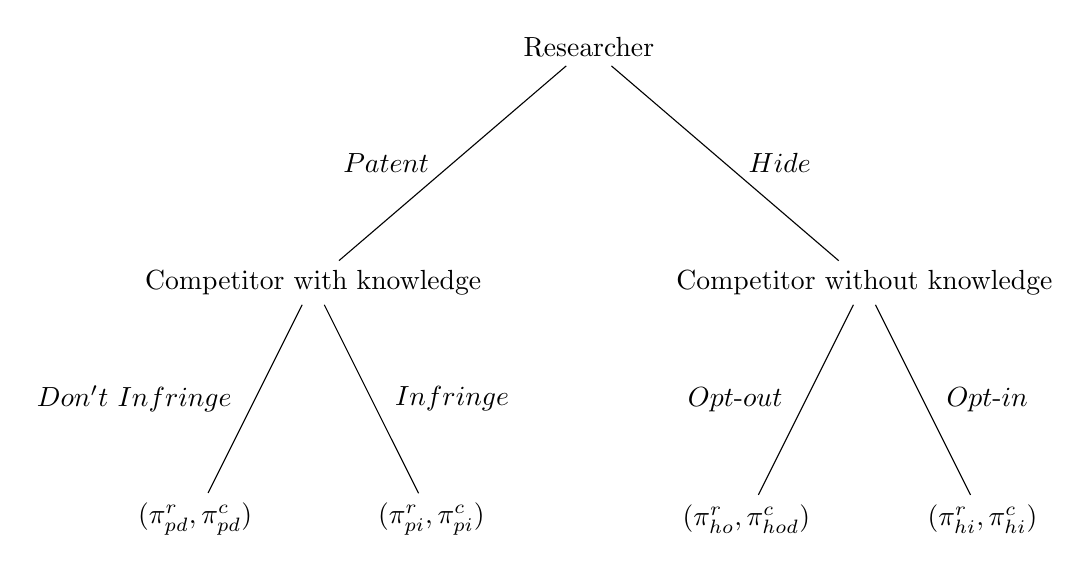
\begin{tikzpicture}[scale=2]
% Specify spacing for each level of the tree
\tikzstyle{level 1}=[level distance=15mm,sibling distance=35mm]
\tikzstyle{level 2}=[level distance=15mm,sibling distance=15mm]
\node(0){Researcher}
child{node{Competitor with knowledge}
child{node{$(\pi^r_{pd},\pi^c_{pd})$}edge from parent[black]node[left,xshift=-5]{$Don't$ $Infringe$}}
child{node{$(\pi^r_{pi},\pi^c_{pi})$}edge from parent[black]node[right,xshift=5]{$Infringe$}}
edge from parent[black]node[left,xshift=-5]{$Patent$} }
child{
node{Competitor without knowledge}
child{node{$(\pi^r_{ho},\pi^c_{hod})$}edge from parent[black]node[left,xshift=-5]{$Opt$-$out$}}
child{node{$(\pi^r_{hi},\pi^c_{hi})$}edge from parent[black]node[right,xshift=5]{$Opt$-$in$}}
edge from parent[black]node[right,xshift=5]{$Hide$}
};
\end{tikzpicture}

The choice between patenting and secrecy can depend on the degree to which the innovation is radical. Firms may prefer to patent less valuable innovations and keep secret the more valuable ones\footnote{See \cite{Anton2004}} , for the simple reason that not disclosing a radical innovation offers more potential for a larger gap between the secret owner and competitors. However, if there are costs to renew the innovation and the degree of innovativeness can affect the probability of receiving the patent, the opposite may be true: high quality projects get patented and lower quality projects do not \citep{Mose2011}. The decision to patent also depends on the competitive gap between the potential patent owner and potential competitors: if the gap is already large, patenting is attractive; if the degree to which the innovation is radical depends on the firms investment, then weak patents are important but stronger patent protection does not necessarily increase innovation \footnote{See \cite{Kultti2006} for details}. %verify!

Perhaps another interesting question to ask is whether a company that can use its patent against someone will always do so. Tentatively, we may say that there may be a cost to enforcing patent rights; but even if that cost is zero, the firm may prefer not to initiate a legal action because the activity in question could be complementary. This kind of market dynamic, where firms willfully choose not to legally enforce their patents, may imply that the system is unnecessary\footnote{For an example of firms not activating their patents in the development of short message services(SMS) see \cite{corrocher2013development}}.
%Elaborate

\subsection{Mechanism Design}

Mechanism design is a natural way to study intellectual property since the system can be said to be designed by legislators from it's inception. The concept of a patent race, where firms invest to achieve a certain technological breakthrough and then only the winner will gain the patent, is indeed equivalent to a contest\footnote{ \cite{Games2003} }. Mechanism design can also shed some light on when it may be optimal not to assign property rights at all. If agents have private information in a bilateral transaction (Coasian setting), the agent with the property right will have an incentive to overstate his cost or value because the other party will not have the option to go to court; whilst if it is unclear who will win in court, parties will have an incentive to tell the truth\footnote{\cite{schmitz2001coase}}.

%check war of attrition

Part of the loss the patent system creates is an allocational efficiency problem. If the highest value user is changing in time, the system has no natural way to prevent the current owner from reaping most of the benefits from a transaction with a higher value user. A natural method for reducing this allocational efficiency is to use the Georgian scheme, and require firms to bid on their own patent every year (a sort of rent). This would establish a price reflecting the current owners value for the patent, and would enable the higher value user to purchase the asset. 

However, the main problem with intellectual property is not the agent who owns the asset but the number of agents who own it. Above all, intellectual property is a monopoly, and as a monopoly it can induce deadweight loss. There are a number of tentative solutions to this: making all patents public (free for anyone to use) is one of them, but the methods are controversial. Suppose a system was instituted where all patents and future patents were bought over by the government at a fixed price. Whilst this would alleviate the deadweight loss problem, due to the variety of project values, two issues would arise. 

The first issue is \textbf{under-rewarding}; projects which are worth more than the posted price would not be undertaken. This would not be a problem if the cost of inventing was below the bought price. The \textbf{under-rewarding} issue would entirely disappear if the consent of the patent owner was required, which transforms the payments into bids. However, for the projects which reject the government fixed bid, this would also entail that their dead-weight loss is still in place\footnote{an interesting historical fact here is that in 18th century France in Lyon, Silk Factory innovation were compensated by the government not only per innovation but also by the dissemination of the idea \cite{foray2013patent}}.

The second issue would be be that projects worth less than the bought value would be \textbf{over-rewarded}. This would naturally create incentives to maximize the number of patents instead of the value added of each invention. A method of alleviating the issue of over-reward would be to choose prices by creating a price system for each patent (allowing firms to bid for each patent\footnote{this method was first suggested by \cite{kremer_1998} and was generalized by \cite{weyl2012market}}). Once the price of the patent is established, the government would then pay that price for the patent. The issue is then: why would a firm bid truthfully if it will not receive the patent? One could indeed imagine that a firm would have the incentive to overbid, and then split the surplus with the patent owner (in the language of game theory, the mechanism is not coalition proof). A partial solution to this problem would be that instead of the government buying out the patent deterministically, it would buy it out with some probability. Unfortunately, this does not alleviate the problem, for the reason that the firms could still make a positive coalition profit in expectation\footnote{\cite{PetersAdamou2018a} show that even firms can exhibit risk avoiding behavior when they partially grow multiplicatively which implies the probabilistic mechanism can be effective}; and if the probability of gaining the asset is low enough, then there would be very little incentive to participate in the mechanism. 

Although generally alleviating the monopoly problem is too difficult, it is possible to play with the time dimension of patents to reduce it. To avoid the coalitional problems, one could devise a mechanism where a patent owner simply bids on its own patent and depending on the amount of the bid, the monopoly granted becomes longer. This mechanism would cause lower productivity sectors to have longer patents, and higher productivity sectors to have shorter duration patents\footnote{ This is because if an industry is innovative the value of the patent will quickly depreciate as more innovative products take over, this means that it would be worthwhile to increase the cost per unit of time for less productive sectors relative to more productive sectors so that the mechanism becomes more truth revealing. This mechanism was created by \cite{Scotchmer1999} and built upon \cite{Cornelli1999}}.

What should the relationship between patent length and the degree of innovation be? For any fixed period patent system, the patent duraction will incentivize projects which can earn sufficient profits within the period. However, the application for patenting may have agents over-applying because it is profitable to gain a patent ex-post on innovations which would not be profitable within the time period. If a patent is granted to these innovations, this would be a pure deadweight loss without an incentive effect. To clarify, the potential for a patent cannot be an incentive for projects which would be ex-ante loss making. But once a project exists, perhaps accidentally, an entrepreneur will still wish for a patent. This means that for the granting process to be effective and not incur accidental deadweight loss, it must use a criterion which has to do with how much profit can be attained within a constrained time period\footnote{\cite{ODonoghue1998}}. \footnote{this class of models is presented with probabilistic enforcement by \cite{Chou2007} }

\subsection{Scope and evidence}

The spike in interest in intellectual property has occurred due to some attacks by economists arguing that such rights should be weakened. The main vanguard of this attack has been in the works of \cite{dosi2006much}, \cite{boldrinlevine} and  \cite{bessen2008patent}. This attack has incited criticism \citep{scherer2009michele} along with responses \citep{boldrin2013s}. The arguments sometimes use specific historical cases to discuss counterfactuals. Perhaps the most radical claim being that James Watts' patent on the steam engine delayed the industrial revolution by decades \citep{boldrinlevine} \citep{nuvolari2004collective}, and similar claims have been made for the development of the plane and the car \citep{merges1994limiting}. One of the most interesting studies on the topic is by \cite{moser2005patent}, who studies historical exhibitions at the crystal palace and conclusively shows that relatively few of the inventions were patented \citep{moser2005patent}\footnote{A similar methodology has been applied to United States fairs, see \cite{khan2013going}}. It seems difficult to evaluate intellectual property as a whole, as the evidence seems mixed\footnote{For evidence that the human genome patent reduced innovation see \cite{williams2013intellectual}}. Surveys with evidence on innovation seem to imply that it is an ineffective policy tool for the majority of industries in the United States, the exception generally being pharmaceuticals and chemicals \footnote{\citep{mansfield1986patents} \citep{levin1987appropriating} replicated by \citep{cohen2000protecting}}. The findings has been similar in Europe \footnote{See \citep{arundel1998percentage}}. 

Take the premise that it is difficult to make sufficient profits from an innovation in some given market. Assume that some level of reward, say x, would balance the losses from the patent system and the incentives for innovation. Now suppose that through time, the market has expanded so that it is easier to gain large portions of profits in a quicker period of time (for instance, as is the case with globalization). If the cost of creating new innovations has remained the same after the market expansion, then the optimal patent system would lower the reward by, say, decreasing patent duration\footnote{this kind of model is presented in \cite{boldrin2009market} }. The intuitive implication is that as the world becomes more globalized, the requirement for patent protection is decreased because the potential payoffs of projects increase. An empirical measurement that could be relevant is the time from discovery to adoption. Ideally, as the adoption times decreases, the length of patent would also decrease \footnote{For evidence about the drop in adoption time see, \cite{comin2006five}}. 

While it is easy to imagine that policy makers optimize a social welfare function, in practice, the system itself relies on a bureaucracy. From an institutional point of view, balancing out incentives is crucial. In this context, if there is not sufficient incentive to reject bad projects, the issue of over-patenting emerges\footnote{see \cite{Caillaud2012} for a model with pooling equilibria with good/bad projects and separating equilibria where only good projects are accepted}(this would naturally emerge as the costs of a welfare reducing patent would be diffuse while the benefits would be narrow). In the American system, court disagreements are discouraged thereby incentivizing institutions to over-grant patents in order to avoid appeals, leads to a sort of patent standards inflation\citep{Masur2011}.

A peculiar empirical fact with implications for patents is the practice of reverse settlements. Reverse settlements, which consist of extending patents by paying other firms not to use a technology, imply a few things about market structure. The simplest implication is that transaction costs must not be very high, so that it is possible for firms to strike Coasian bargains. Since these contracts are firm specific, the empirical implication is that smaller firms do not matter enough to change the profitability of such arrangements. The scope of reverse settlements is unknown, but if these contracts are possible before the creation of an innovation, it may imply that a large segment of the patent system is unnecessary, since firms can simply negotiate ex-ante with the limited number of firms who could use it. The ability to patent could then be interpreted as an increase in the bargaining power of the first firm \citep{Green1995}. It is interesting to ponder if firms can foresee whether this bargain will occur: if firms do not have this capacity but undertake the investment anyway, it must be expected that patents over-reward.

An alternative explanation for reverse settlements is that patents are, in practice, probabilistic, and firms do not want to take the risk of a court failing to validate their patent. This probabilistic feature can have two effects: it can protect innovations which upon closer scrutiny, would not be protected. It can lead to firms to pursue secrecy strategies\footnote{For details about probabilistic enforcement see, \cite{Lemley2005}, to see how reverse settlements can signal invalid patents, see \cite{Dolin2011}}.

Perhaps the strangest empirical regularity is the practice of patent pooling. Firms jointly agree to enter a patent coalition and agree not to enforce their patent within that pool. This kind of structure inevitably leads to a standard for entering the patent pool, where entry will be granted only if one has a sufficiently important patent to the coalition. What is interesting is that this may create incentives for achieving this standard. However once in the pool, there may be little reason to keep innovating. Still, even without these dynamic notions, the presence of a patent pool may be welfare reducing if technologies are not complementary. \footnote{see \cite{Lerner2004}}

This section on intellectual property has discussed various economic arguments justifying the legal practice. We have discussed when a firm may wish or may not wish to enforce it's patent, this is related to the first chapter, where it shown that when a firm has an intellectual asset, it may not wish to enforce its claim rights on all agents because value could emerge as a function of number of agents consuming. Perhaps most importantly, we have discussed the two fundamental assumptions that run through most of the economic literature. Foreseeability is relevant to chapter 3 in this thesis as it focuses on agents maximizing growth. This growth heuristic allows for agents to fit into evolutionary environments such as those described above. In other words, the growth heuristic is about agents surviving in the long run, not about deducing the expected value of pursuing a certain project. 

\newpage

\section{Contrbutions in this thesis}

\subsection{First chapter}

The first chapter is a contribution to the economic modeling of pricing in an environment where a firm has a monopoly and agents value consuming as a group, a network good. The good in question is assumed to be an intellectual asset implying that the marginal cost to the firm of producing an additional unit is zero. Whilst most of the network goods in the literature implicitly assume that the intrinsic quality of the product increases as the number of consumers increases, the model switches where the value-added comes from, specifically the product value is extrinsic value. This implies that the increase of the value of the good emerges from the demand side. The main result of the paper is that if a firm has a monopoly on a good, and there exists two ways a product can be sold, a firm will opt into giving to the lower tiered consumers for free. The implication is that rights pertaining to intellectual property should be centralized, in the sense that if the firm has the right to exclude other firms, it should also have the right to exclude users. The result goes against the way in which current court systems categorize piracy, mainly as a criminal offense. Categorizing piracy as a criminal offense implies that the firm does not have claim rights and can result in non pareto optimal equilibria. 

The abstract of the paper is as follows: This paper presents a model for the consumption of a \textit{cultural} good where consumers can either purchase or pirate the good (or not consume it). Because of the specificity of the \textit{cultural} good, active consumers (users), buyers and pirates, derive a network utility that depends on the numbers of users of the goods with which they can share their experience of the cultural good. It is shown that the monopoly firm selling the cultural good may obtain a higher profit when piracy is possible than when it is not. Consequently, it is presented that increasing the cost of piracy has a non monotonic effect on a firm's profit and welfare.

\subsection{Second chapter}

The second chapter studies the choice of innovation in the presence of buyouts. The model can be interpreted as being within the incomplete contracts literature as firms cannot contract ex-ante. We present a two firm setting model with an entrant and incumbent where the entrant selects a technology. The choice of technologies is a sequential innovation and a radical one. We find that the ability to buyout affects the direction of innovation towards sequential innovations, that is, there exist cases where if no buyouts can occur, the radical innovation would have been pursued but the option to buyout creates a preference reversal. This effect only exists if the entrant has bargaining power. We show that this holds for both Bertrand and Cournot Competition. Finally we discuss the welfare implications of buyouts in this two technology paradigm and the link to the Coase theorem. 

We give a brief numerical example here to illustrate: 
\subsubsection{Numerical example with two time periods}


We have two time periods with the entrant selecting which innovation to pursue. The sequential technology will give the entrant the intermediate technology in period 1 and the advanced technology in period 2. The radical innovation will simply probabilistically give the advanced technology every period. 

The profit of the entrant with the advanced technology is given by, $40$. The profit of the incumbent with the advanced technology is given by $100$. Additionally, let the profit of the incumbent when competing with an intermediate technology be $20$, whilst the profit of the incumbent with the initial technology without competition is: $=80$. Finally, we assume a Nash bargaining solution where firms have equal bargaining power, $.5$ and that the radical innovation has a $50$\% chance of succeeding. 

We first do the case where there are no buyouts. If no buyouts do occur and the entrant chooses the sequential innovation then the entrant will earn, $40$, which will only be realized in the second period. If the entrant chooses the radical innovation the payoff will be $.5(40+40)+(.5)^2(40)=50$. Since $50>40$, if no buyout occurs the radical innovation will be chosen. 

If buyouts do occur then the incentives change. The Nash surplus for the sequential innovation is, $NS_s = 100+80-20-40=120$. Therefore the payoff of the entrant after bargaining is $40+\frac{1}{2}(120)=100$. The radical innovation surplus is similarly $NS_r = .5(200)+(.5)^2 180+(.5)^2 160-(.5)^2 80-(.5)^2-50=75$. Therefore the payoff after bargaining $50+\frac{1}{2}(75)=87.5$ so the entrant pursues the sequential innovation. 

 \subsection{Third chapter}

Whilst working on the second chapter this author noticed that firms were preferring earlier payments to later payment without an explicit discount rate. After some tinkering on the subject this led to the identification of the cause as coming from the multiplicative dynamic used. This dynamic was later removed from the second chapter and became its own project, the third chapter. Whilst the chapter focuses on agents discounting, the method used abstracts away from any subjectivity in the discount rate. Meaning that the discount rate could be interpreted as pertaining to the optimal long term use of objects in specific environments. This means that the theory can be directly applied for assets.  

The problem question is about discounting. Specifically, in laboratory experiments agents discount the future in different ways. The two main kinds of discounting reported on are exponential and hyperbolic. Economists then try to conjure up reasons as to why the different sort of discounting may occur. There are essentially three approaches: psychological, agents ignore some information in some contexts; informational, agents have a specific information structure that causes the behavior; axiomatic, agents have a specific method of reasoning that implies this behavior. 

These theories posit an initial behavior and explain the discounting behavior. The problem with this approach is that an explanation for the initial behavior is not given. Why do agents ignore some information, why do agents have this specific (usually bayesian) information structure and why do agents have these axioms? If these theories are just different languages of describing the same behaviors then there is no issue, however it is quite clear that there will be circumstances where their predictions will not overlap. 

The approach used in this paper appeals to consilience, that is, an axiom that is already used in another field, evolutionary theory. The axiom in question is growth, agents will simply maximize their growth, it is common sense why this axiom would naturally rise when evolutionary forces are at work. Simply, agents will maximize growth because agents who did not maximize growth would not be around in the long run\footnote{Assuming random mixing}. The growth axiom allows the explanation to be on physical environmental level instead of being an explanation about cognition. 

% It is perhaps worth saying a few words about the importance of uniqueness. The scientific endeavour aims to predict a single value for each state. Take a pendulum as an example, if the description of the pendulum includes only its angle, this will not yield a single prediction, an angle of 60\% may map into an angle of 90\% or 180\% after one second. However if by the 'state' of the pendulum we include not only its current angle but its angular velocity and material we will instantly explain over 90\% of the variation. In other words, the less values are predicted, the more the system under description is scientific. It is also imperative that the variables used in the state are measurable. 


 % question pursued is how agents in different circumstances discount future payouts. This chapter is the one with the widest scope as it is a simple alternative way to frame decision theory. Most explanations of discounting rely either on endogenous preferences for discounting, psychological effects or incomplete information. The chapter offers an alternative view which recovers all the traditional methods of discounting(hyperbolic and exponential) by assuming agents have a simple growth decision rule. This kind of decision theory is innovative in that it does not take a descriptive position on an agents knowledge or decision making abilities, but instead just describes the kind of environment the agent is in and how that environment can best be exploited. This is an example of the kind of heuristics that can emerge if we consider moving away from frameworks which are too reliant on agents ability to deduce.

The abstract of the paper is as follows: An important question in economics is how people choose between different payments in the future. The classical normative model predicts that a decision maker discounts a later payment relative to an earlier one by an exponential function of the time between them. Descriptive models use non-exponential functions to fit observed behavioral phenomena, such as preference reversal. Here we propose a model of discounting, consistent with standard axioms of choice, in which decision makers maximize the growth rate of their wealth. Four specifications of the model produce four forms of discounting -- no discounting, exponential, hyperbolic, and a hybrid of exponential and hyperbolic -- two of which predict preference reversal. Our model requires no assumption of behavioral bias or payment risk.


%\section{Introduction to chapters}%

%The first article aims to show that even if it is desirable to give a monopoly on a good, this does not entail that property rights should also be used against consumers.%

%The second article uses the coase theorem but shows that the ability to negotiate for the buyout of innovations causes firms to pursue innovations that increase externalities.%

%The third article is a general model of discounting, the aim of this paper is to show that it is possible to define discounting as something other than a preference, under this interpretation, the %choices entrepreneurs make is not a function of their preferences but a function of their environment.

%%%%%%%%%%%%%%%%%%%%%%%%%%%%%%%%%%

%To take an example, suppose that some person can produce k units if he were to work on a specific asset. Suppose there are 10 assets and 20 citizens. The citizens own assets equally, so each citizen owns $5 \%$ . If a citizen can work on a specific asset to produce 20 units of a good, then he will only receive 1 of those goods in the end. Which means his willingness to expend effort is 1. If on the other hand, the assets are redistributed in such a way that every citizen still owns $5 \%$ but the citizens own higher shares of the assets they work on, if for example that same citizen had $10\%$ share of the asset he worked on then, his willingness to expend effort had doubled. In other words, we can say that the distribution of ownership does NOT matter if every citizen works on every asset and their productivity of every citizen is the same.



%To make ownership of an asset illegal is to make its market value zero or negative.

%The Coasian view of property rights claims that allocative efficiency is in fact irrelevant as long as there are no transaction costs and bargaining is possible.

%The question of what assets property rights protects can be quite complex. Some possible categories to consider, are tangible vs intangible; the ratio of subjective value to market value. One could also have alienable versus inalienable. Or one could define assets as having market value, in this formulation an asset only acquires property rights when it has accumulated sufficient components to acquire either subjective or market value. The market value component could also be used to justify the scope of protection.

%Note that positive market value exists only if at least one non-possessor of the good has a subjective value for it. If the only person with positive subjective value of the good acquires it, then by definition the good no longer has market value. It is also possible for a good to have negative market value or subjective value. If the possessor of the good has a negative subjective value of the good AND no property rights to it, then the person is likely to either destroy it or abandon it.

%I%f a good only has value for a single person, then it has no market value. If it has value for more than a single person then it does have market value. ue

%\subsection{Externalities}

%To define the Coase theorem we need the concept of externalities. Externalities are usually defined on a set of actions, it is when an action of A, has an effect on anybody else but A. Contracts can be framed as trying to create incentives for positive externalities, in other words to increase the payoff of an agent by A by taking a specific action.

%If an agent tries to

%\subsubsection{Coasian}




%The coasian view of property rights aims to explain or justify property through two categories. Transaction costs and negative externalities. The Coasian approach has a simple statement of the form: externalities will only matter if transaction costs are large.

%If ownership and possession are not identical, this creates the possibility of temporary transfer of assets to higher value users or to lower cost producers. Similarly there is the investment efficiency from stable ownership, this is asset related skills.

%The value of assets is not only direct, it can be expected to increase the value of other assets that are complementary to the asset itself.

%There is also of course a subjective value from ownership. For instance, suppose an owner who does not intend to use the asset but intends to rent it forever. If this owner discounts, the asset merely represents a series of cash flows, for which he should able to exchange a lump sum for. If we suppose that someone prefers to own rather than rent, liquidity is only constraint for transfer to occur.

%Economies of scope between monitoring and apprehension.